\documentclass[11pt]{article}
\usepackage[T1]{fontenc}
\usepackage[utf8]{inputenc}
\usepackage{lmodern,microtype}
\usepackage[margin=1in]{geometry}
\usepackage{amsmath,amssymb,amsthm,mathtools}
\usepackage{graphicx,booktabs,array,longtable}
\usepackage[dvipsnames]{xcolor}
\usepackage{enumitem}
\usepackage{fancyhdr}
\usepackage{xurl}
\usepackage[colorlinks=true,linkcolor=MidnightBlue,citecolor=MidnightBlue,urlcolor=MidnightBlue]{hyperref}
\hypersetup{pdftitle={Extreme contributions and a functional bridge under small spectral totals},pdfauthor={Research note prepared for Vladimir Reshetnikov}}
\newtheorem{theorem}{Theorem}[section]
\newtheorem{lemma}[theorem]{Lemma}
\newtheorem{proposition}[theorem]{Proposition}
\newtheorem{corollary}[theorem]{Corollary}
\theoremstyle{definition}
\newtheorem{definition}[theorem]{Definition}
\theoremstyle{remark}
\newtheorem{remark}[theorem]{Remark}
\setlist[enumerate]{leftmargin=*,itemsep=4pt}
\setlist[itemize]{leftmargin=*,itemsep=3pt}
\setlength{\emergencystretch}{3em}
\setlength{\headheight}{14pt}
\pagestyle{fancy}
\fancyhf{}
\fancyhead[L]{\small Conditional spectral extremes}
\fancyhead[R]{\small 27 November 2026}
\fancyfoot[C]{\thepage}
\renewcommand{\headrulewidth}{0.3pt}
\title{\vspace{-1.5em}\textbf{Extreme contributions and a functional bridge\\under small spectral totals}\\[0.6em]
\large A marked Poisson limit and a second height scale\\for completed Dirichlet $L$-functions}
\author{Research note prepared for Vladimir Reshetnikov}
\date{27 November 2026}
\begin{document}
\maketitle
\begin{abstract}
The ProveIt GRH article studies random gamma weights attached to a deterministic
zero spectrum and conditioned to have a very small weighted sum. We extend its
conditional spectral laws in two directions. For every spectrum with a regularly
varying counting function of index $\alpha$, and every exponent $p>\alpha$, we
prove a marked Poisson limit for the largest individual contributions. Their
spectral locations occur at height $u/(\log N(u))^{1/p}$, below the bulk scale $u$;
the $p$th power of a normalized location has a $\mathrm{Gamma}(\alpha/p,1)$ law,
independent of the gamma shape of the weights. We also prove convergence of the
entire centered bulk process to a Brownian bridge, jointly independent of the
extreme process and the exponential boundary slack. For completed Dirichlet
$L$-functions the winning height has a half-normal limit on the scale
$u/\sqrt{\log u}$. With probability tending to one, every fixed number of largest
contributions lies in a band carrying a vanishing fraction of the total mass.
For exponential weights, a heat-trace formula also gives an effective
enclosure of the centering constant from a two-term counting estimate.
The probabilistic theorems are unconditional; Dirichlet GRH identifies the
associated Laplace transform with a reciprocal completed $L$-function.
Complete proofs, a source comparison, independent finite numerical checks,
and reproducible experiments are provided.
\end{abstract}

\section{Contribution and relation to the source}

\subsection{The concrete Dirichlet conclusion}

Let $\gamma_1,\gamma_2,\ldots$ be the positive ordinates of the nontrivial
zeros of the Riemann zeta function, counted with multiplicity. Give each
occurrence an independent mean-one exponential weight $E_j$, and set
\[
 X=\sum_{j\ge1}\frac{E_j}{\gamma_j^2}.
\]
Condition on $X\le x$ and let $x\downarrow0$. Define the exact saddle $u>0$ by
\[
 x=\sum_j\frac1{\gamma_j^2+u^2}.
\]
Let $M=\max_j E_j/\gamma_j^2$ and let $I$ be the almost surely unique
maximizing index. The results proved below give, with
\[
 b_0(u)=\log u+\frac12\log\log u-\log(4\sqrt\pi),
\]
the joint limit
\begin{equation}\label{intro:eq:limit}
 \left(u^2M-b_0(u),\ \frac{\sqrt{\log u}\,\gamma_I}{u},\ u^2(x-X)\right)
 \Longrightarrow (G,Z,E).
\end{equation}
The three variables on the right are independent and have laws
\[
 \mathbb P(G\le z)=e^{-e^{-z}},\qquad
 f_Z(y)=\frac2{\sqrt\pi}e^{-y^2}\mathbf1_{y>0},\qquad
 \mathbb P(E>y)=e^{-y}\quad(y\ge0).
\]
Here $Z$ has the law of the absolute value of a centered normal variable
of variance $1/2$. The limit concerns the added random weights, not a
randomness assumption on the zeros.

The cumulative mass at heights at most $cu$ tends to
$A(c)=2\arctan(c)/\pi$. Thus about half the mass lies below height $u$,
whereas the largest contribution occurs at height of order
$u/\sqrt{\log u}$. More sharply, take
$h=u/(\log u)^{1/4}$. For every fixed $k$, the largest $k$ contributions
all lie below $h$ with probability tending to one, although
\[
 \frac{\sum_{\gamma_j\le h}E_j/\gamma_j^2}{X}\longrightarrow0,
 \qquad \frac{M}{X}\sim\frac4u
\]
in conditional probability. The largest terms concentrate in a part of
the spectrum that carries asymptotically none of the total mass.

\begin{figure}[ht]
\centering
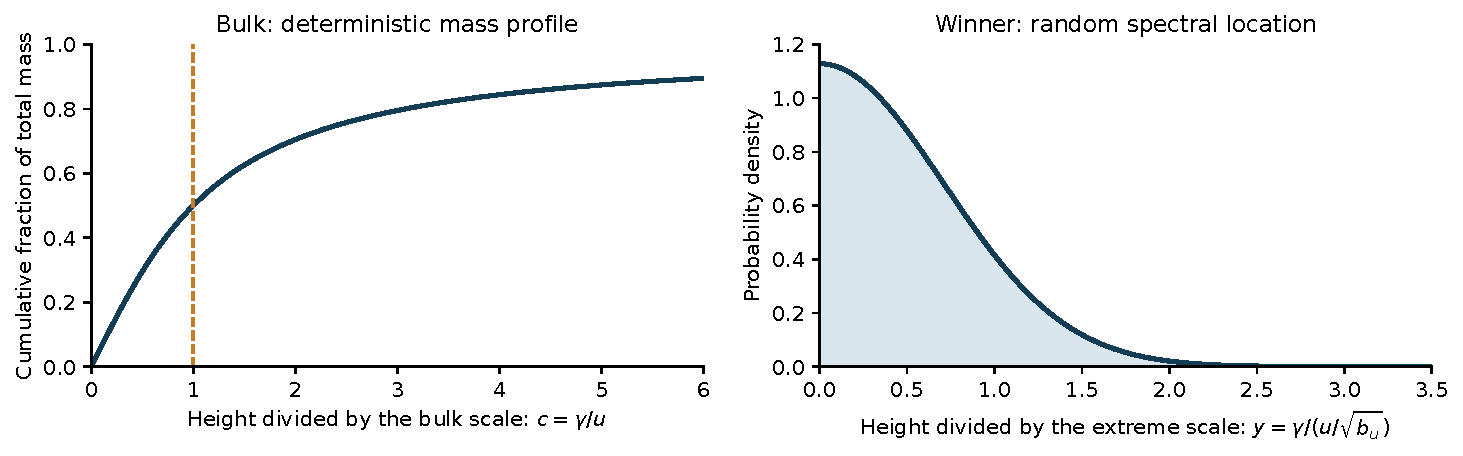
\includegraphics[width=\textwidth]{figures/two_scales.pdf}
\caption{Two different limiting descriptions. The left panel measures total
mass on the height scale $u$. The right panel measures the location of the
largest contribution on the smaller height scale $u/\sqrt{b_u}$, where
$b_u\sim\log u$. The two horizontal axes have different units.}
\label{fig:scales}
\end{figure}

The general theorem also determines every fixed number of largest terms,
allows arbitrary gamma shape $\theta>0$, and applies to any positive
spectrum with regularly varying count. A second theorem promotes the
source's finite-dimensional Gaussian limits to convergence of the entire
bulk path. That path, the extreme point process, and the boundary slack
have mutually independent limits.

\subsection{What was inspected and what is new}

The source snapshot is ProveIt commit
\texttt{00cadb961bbe77c74e5d082c4948f8884d58a970}. Its GRH directory indexes
an article merging 184 research reports and ten additional packets awaiting
integration~\cite{ProveIt2026}. The article explicitly describes itself as a
merge rather than an independent verification. We examined the source
theorem interface, the article index and source sections, the recent-packet
descriptions, and in detail the conditional spectral laws in
\texttt{Article/sections/ana.tex}.

The upstream arithmetic input is RH and GRH for Dirichlet $L$-functions,
as exported by the vendored \texttt{grh-lean} revision
\texttt{72fead102f663d5c7a407964a13dc0cf9d977207}. Its five exported statements
and reported independent kernel checks are documented in the source and
Sutherland's verification record~\cite{Sutherland2026}. We use that input
in precisely the scope stated in the source. The new probability proofs
below do not depend on repeating that build.

\begin{center}
\begin{tabular}{@{}p{0.43\textwidth}p{0.50\textwidth}@{}}
\toprule
Inspected predecessor & Additional conclusion proved here\\
\midrule
\texttt{ana:thm:condlaw}: finite bulk cutoffs and fixed low coordinates
& Full bulk process in $D[0,1]$, jointly with the extremes.\\[5pt]
\texttt{ana:thm:block}: independence on blocks $h=o(u)$ with tilted rates
& Marked Poisson limit on the moving scale $u/(\log N(u))^{1/p}$.\\[5pt]
\texttt{ana:thm:medianheight}: height carrying half the mass
& Random location of the largest individual terms and localization in a
band of vanishing mass.\\[5pt]
Classical gamma maxima and small-norm conditioning
& A location-marked limit for an infinite, nonidentically weighted spectrum
under rare conditioning.\\
\bottomrule
\end{tabular}
\end{center}

Gamma maxima and Gumbel limits are classical; see Bose, Dasgupta and
Maulik~\cite{Bose2008}. Small Gaussian ellipsoids and conditional moments
were studied by Mayer-Wolf and Zeitouni~\cite{MayerWolf1993}. For
unconditioned spectral maxima, Gy\"orgyi,
Holdsworth, Portelli and R\'acz~\cite{Gyorgyi2003} study extremal Fourier
intensities with power-law rates. The small-total constraint and the
marked location process considered here are additional features. The contribution
here is the combined spectral location law, its scale, and its independence
from the entire conditional bulk bridge and slack. A targeted literature
comparison did not locate this precise statement. This establishes a
specific extension of the inspected work, not an exhaustive historical
priority claim.

\paragraph{Proof status.}
The mathematical arguments are supplied below, including the local limit,
conditioning, infinite-tail, and path-tightness steps. Independent numerical
checks support implementation consistency. No Lean formalization of these
new theorems is claimed. Constants and asymptotics are for fixed
$\theta,p,\alpha$ and a fixed spectrum; no uniformity in growing conductor or
degree is asserted.

\medskip
\noindent\textbf{Organization.} Section~\ref{sec:extremes} proves the marked
extreme law and the Dirichlet specialization. Section~\ref{ext:sec:functional}
proves the functional bridge extension. Section~\ref{sec:computation}
describes exact finite identities and numerical validation. The final
section records a formalization route and the remaining quantitative questions.

% Self-contained mathematical section. Requires amsmath, amssymb, amsthm.
% All limits of marked point processes and their marks are weak limits, not TV limits.
% Exact gamma convention: Gamma(shape, rate).

\section{Extremes under a small-total constraint}
\label{sec:extremes}

The preceding spectral-conditioning results describe fixed coordinates and
macroscopic bands.  Extremes live at a different height.  The theorem below
identifies that height, the largest contributions, and their joint relation
to the bulk fluctuations and to the distance from the conditioning boundary.

\subsection{Assumptions and exact normalization}

Let $\theta>0$, $p>\alpha>0$, and let $(\gamma_j)_{j\ge1}$ be a locally
finite multiset of positive numbers tending to infinity.  Repetitions are
allowed and are counted separately.  Assume that
\[
 N(T)=\#\{j:\gamma_j\le T\}\quad\hbox{satisfies}\quad
 \frac{N(cT)}{N(T)}\longrightarrow c^\alpha\qquad(c>0).
\]
Thus $N$ is regularly varying of index $\alpha$; we use the standard uniform-convergence and summation properties in~\cite{BGT1987}.  Let $G_j$ be independent
gamma random variables of shape $\theta$ and rate one and put
\[
 X=\sum_{j\ge1}\frac{G_j}{\gamma_j^p}.
\]
The sum is finite almost surely, since $p>\alpha$ implies
$\sum_j\gamma_j^{-p}<\infty$.
For sufficiently small $x>0$, define $t=t_x>0$ uniquely by
\begin{equation}\label{ext:eq:saddle}
 x=\theta\sum_j\frac1{\gamma_j^p+t},\qquad u=t^{1/p}.
\end{equation}
The right side is continuous, strictly decreasing from $\mathbb E X$ to
zero.  In particular, $u\to\infty$ as $x\downarrow0$.
Write
\[
 R_{j,u}=\frac{tG_j}{\gamma_j^p},\qquad
 S_u=\sum_jR_{j,u}=tX,\qquad \mu_u=tx,
 \qquad Y_x=t(x-X).
\]
The slack $Y_x$ is nonnegative under the conditioning $X\le x$.

For $a>0$ let
\[
 Q_\theta(a)=\frac1{\Gamma(\theta)}
       \int_a^\infty s^{\theta-1}e^{-s}\,ds
\]
be the gamma survival function.  Define $b=b_u$ as the unique positive
solution of
\begin{equation}\label{ext:eq:exactb}
 \Lambda_u(b):=
 \sum_j Q_\theta\bigl(b[1+(\gamma_j/u)^p]\bigr)=1,
 \qquad v=v_u=\frac{u}{b_u^{1/p}}.
\end{equation}
For every positive argument this series converges, uniformly on compact
subsets of $(0,\infty)$.  It is continuous and strictly decreasing, tends
to infinity at zero and to zero at infinity; hence the definition is
unambiguous.

Let $\nu_{\alpha,p}$ be the probability law on $(0,\infty)$ with density
\begin{equation}\label{ext:eq:mark}
 \nu_{\alpha,p}(dy)=
 \frac{p}{\Gamma(\alpha/p)}y^{\alpha-1}e^{-y^p}\,dy.
\end{equation}
Equivalently, $Z\sim\nu_{\alpha,p}$ if and only if
$Z^p\sim\mathrm{Gamma}(\alpha/p,1)$.

\begin{theorem}[Conditional marked-extreme law]\label{ext:thm:main}
Under the assumptions above, the following statements hold.
\begin{enumerate}
\item The exact centering satisfies
\begin{equation}\label{ext:eq:basymp}
 b_u\sim\log N(u),\qquad
 \frac{\Gamma(1+\alpha/p)}{\Gamma(\theta)}
       N(v_u)b_u^{\theta-1}e^{-b_u}\longrightarrow1.
\end{equation}
\item Conditionally on $X\le x$, the marked point process
\begin{equation}\label{ext:eq:pointprocess}
 \mathcal P_x=\sum_{j\ge1}
       \delta_{(R_{j,u}-b_u,\,\gamma_j/v_u)}
\end{equation}
converges to a Poisson point process $\mathcal P$ of intensity
\[
 e^{-z}\,dz\,\nu_{\alpha,p}(dy).
\]
The convergence includes the finite collection of atoms above any fixed
level in the first coordinate, after tails of the mark coordinate are
removed and then restored by tightness.  Jointly,
$Y_x\Rightarrow E_0$, where $E_0$ is exponential of rate one and independent
of $\mathcal P$.
\item Order the contributions decreasingly as
$R_{I_1,u}>R_{I_2,u}>\cdots$.  For every fixed $k$,
\begin{equation}\label{ext:eq:topk}
 \left(
   \left(R_{I_i,u}-b_u,\,(\gamma_{I_i}/v_u)^p\right)_{i=1}^k,
   Y_x
 \right)
 \ \,\Longrightarrow\ \,
 \left(
   \left(-\log(E_1+\cdots+E_i),\,H_i\right)_{i=1}^k,
   E_0
 \right),
\end{equation}
where $E_0,E_1,\ldots$ are independent unit-rate exponentials,
$H_1,H_2,\ldots$ are independent $\mathrm{Gamma}(\alpha/p,1)$ variables,
and the two families are independent.  In particular,
\[
 \mathbb P\!\left(\max_jR_{j,u}-b_u\le z\mid X\le x\right)
 \longrightarrow \exp(-e^{-z}).
\]
The limit of the maximizing height is independent of this Gumbel
fluctuation and of the slack.
\end{enumerate}
\end{theorem}

The conclusion concerns the random weights $G_j$.  It makes no assertion
that the deterministic numbers $\gamma_j$ are themselves random,
independent, simple, or separated.  In particular, convergence of the
marks is weak convergence: their finite-$u$ distributions are discrete,
whereas \eqref{ext:eq:mark} is continuous.

\subsection{Exponential tilting and local limits}

Put
\[
 K(t)=\theta\sum_j\log(1+t/\gamma_j^p),\qquad
 \frac{d\mathbb P_t}{d\mathbb P}=e^{-tX+K(t)},\qquad
 a_{j,u}=\frac1{1+(\gamma_j/u)^p}.
\]
Integrating out the independent tail shows that under $\mathbb P_t$ the
$R_{j,u}$ are independent gamma variables of shape $\theta$ and rate
$a_{j,u}^{-1}$.  Thus
\[
 \mathbb E_tS_u=\mu_u=\theta\sum_j a_{j,u},\qquad
 \sigma_u^2=\operatorname{Var}_tS_u
             =\theta\sum_j a_{j,u}^2.
\]
For $r>\alpha/p$, define
\begin{equation}\label{ext:eq:Cr}
 C_r=\int_0^\infty
       \frac{\alpha y^{\alpha-1}}{(1+y^p)^r}\,dy
     =\frac{\Gamma(1+\alpha/p)\Gamma(r-\alpha/p)}{\Gamma(r)}.
\end{equation}
In particular, $C_2=(1-\alpha/p)C_1$.

\begin{lemma}[Spectral sums]\label{ext:lem:sums}
For every $r>\alpha/p$,
\[
 \sum_j a_{j,u}^r\sim C_rN(u).
\]
The same statement, with the integral restricted accordingly, holds for
a fixed interval $\gamma_j/u\in(c,d]$, where $0\le c<d\le\infty$.
Consequently $\mu_u\sim\theta C_1N(u)$ and
$\sigma_u^2\sim\theta C_2N(u)$.
\end{lemma}

\begin{proof}
The counting measures
$N(u)^{-1}\sum_j\delta_{\gamma_j/u}$ converge on compact subintervals of
$(0,\infty)$ to $\alpha y^{\alpha-1}dy$.  The mass below a fixed
$\varepsilon$ tends to $\varepsilon^\alpha$.  At infinity, regular
variation gives, for any sufficiently small $\eta>0$, an eventual bound
$N(2^ku)/N(u)\le A_\eta2^{k(\alpha+\eta)}$.  Splitting the tail into
dyadic intervals bounds it by a convergent geometric series because
$pr>\alpha+\eta$.  This proves convergence of the integrals.
The substitution $s=y^p$ gives the beta integral in
\eqref{ext:eq:Cr}.
\end{proof}

Write $\varphi_\lambda$ for the centered normal density of variance
$\lambda>0$ and $\varphi=\varphi_1$.

\begin{lemma}[Local limits with deleted coordinates]\label{ext:lem:llt}
The standardized sum $(S_u-\mu_u)/\sigma_u$ has, for all sufficiently
large $u$, a bounded continuous density $f_u$, and
$f_u\to\varphi$ uniformly and in $L^1$.
The same conclusion holds after deleting all coordinates
$\gamma_j\le h(u)$ whenever $h(u)=o(u)$, with the remaining sum centered
at its own mean and still divided by $\sigma_u$.
After deleting an arbitrary single coordinate $j$, convergence is
uniform both in the argument of the density and in $j$.
More generally, a sum restricted to a fixed spectral band, centered at
its own mean and divided by $\sigma_u$, has a density converging uniformly
and in $L^1$ to the centered normal density with the variance prescribed
by Lemma~\ref{ext:lem:sums}.
\end{lemma}

\begin{proof}
For any of the indicated sums, its centered characteristic function is
\[
 \phi_u(s)=\prod_{j\in J_u}
       e^{-is\theta a_{j,u}/\sigma_u}
       (1-is a_{j,u}/\sigma_u)^{-\theta}.
\]
For fixed $s$, Taylor expansion gives
\[
 \log\phi_u(s)=
 -\frac{\theta s^2}{2\sigma_u^2}\sum_{j\in J_u}a_{j,u}^2
 +O_{\theta,s}(\sigma_u^{-1}),
\]
since $0<a_{j,u}\le1$.  Deleting a singleton changes the variance fraction
by at most $\theta/\sigma_u^2$, uniformly in the index.  Deleting a lower
block with $h=o(u)$ changes it by at most
$\theta N(h)/\sigma_u^2=o(1)$.  The latter assertion follows by first
bounding $h\le\varepsilon u$ and then sending $\varepsilon\downarrow0$.

Choose a compact interval contained in the retained spectral band;
for the full sum or a deleted lower block one may use $[u,2u]$.
It contains at least $cN(u)$ retained coordinates, each satisfying
$a_{j,u}\ge c'>0$.  A singleton deletion does not affect this conclusion.
Writing $n=N(u)$, constants $A,B>0$ therefore give
\[
 |\phi_u(s)|\le(1+As^2/n)^{-Bn}.
\]
For $|s|\le\sqrt n$ this is bounded by $e^{-cs^2}$; the integral for
$|s|>\sqrt n$ tends to zero exponentially in $n$ after $s=\sqrt n\,r$.
The characteristic functions consequently converge in $L^1$, uniformly
in the index for singleton deletion.  Fourier inversion gives uniform
convergence of densities.  Their integrals are one, so Scheffe's lemma
gives $L^1$ convergence.  The proof for each fixed band is identical.
\end{proof}

Let $\mathbb Q_x=\mathbb P(\,\cdot\mid X\le x)$ and set
\[
 D_u=\mathbb E_t\bigl[e^{S_u-\mu_u}\mathbf1_{S_u\le\mu_u}\bigr].
\]
The conditioning event has positive probability: choose a finite initial
segment with expected tail below $x/4$, use Markov's inequality on the
tail, and require all terms of the initial segment to be sufficiently
small.  The exact change of measure and the local limit give
\begin{equation}\label{ext:eq:D}
 \frac{d\mathbb Q_x}{d\mathbb P_t}
       =D_u^{-1}e^{S_u-\mu_u}\mathbf1_{S_u\le\mu_u},\qquad
 \sigma_uD_u=\int_0^\infty e^{-y}f_u(-y/\sigma_u)\,dy
       \longrightarrow\varphi(0).
\end{equation}

\begin{lemma}[Mesoscopic independence and uniform marginal domination]
\label{ext:lem:conditioning}
Let $B_u=\{j:\gamma_j\le h(u)\}$ with $h=o(u)$, and let $P_{B,u}$ be
the product law of $(R_{j,u})_{j\in B_u}$ under $\mathbb P_t$.
Then
\begin{equation}\label{ext:eq:blockTV}
 d_{\rm TV}\!\left(
   \mathcal L_{\mathbb Q_x}((R_{j,u})_{j\in B_u},Y_x),
   P_{B,u}\otimes\mathrm{Exp}(1)\right)\longrightarrow0.
\end{equation}
Moreover, for all sufficiently large $u$, every index $j$ and every
Borel set $A\subseteq(0,\infty)$,
\begin{equation}\label{ext:eq:marginaldom}
 \mathbb Q_x(R_{j,u}\in A)\le2\mathbb P_t(R_{j,u}\in A).
\end{equation}
The constant two can be replaced by $1+o(1)$ uniformly in $j$ and $A$.
\end{lemma}

\begin{proof}
Let $S_B=\sum_{B_u}R_{j,u}$, $\mu_B=\mathbb E_tS_B$, and let $g_u$ be
the density of the centered complementary sum divided by $\sigma_u$.
Relative to $P_{B,u}\otimes\mathrm{Exp}(1)$, the joint law in
\eqref{ext:eq:blockTV} has the exact density
\begin{equation}\label{ext:eq:RNblock}
 L_u(r,y)=\frac1{\sigma_uD_u}\,
   g_u\!\left(-\frac{\sum_{B_u}r_j-\mu_B+y}{\sigma_u}\right).
\end{equation}
Indeed, the complementary sum must be $\mu_u-\sum r_j-y$ and the
Jacobian for its standardized density is $1/\sigma_u$.
Under the reference law,
$\operatorname{Var}_tS_B\le\theta N(h)=o(\sigma_u^2)$, and $y$ has
mean one.  Thus the argument of $g_u$ tends to zero in probability.
Lemma~\ref{ext:lem:llt} and \eqref{ext:eq:D} imply $L_u\to1$ in
probability and give a uniform bound on $L_u$.  Hence
$\mathbb E|L_u-1|\to0$, proving \eqref{ext:eq:blockTV}.

For a singleton, use \eqref{ext:eq:RNblock} with the singleton-deleted
density and integrate over $y$.  Its supremum converges to $\varphi(0)$
uniformly in the deleted index, while $\sigma_uD_u\to\varphi(0)$.
The resulting marginal likelihood ratio is bounded by $1+o(1)$
uniformly in its argument and index.  This gives
\eqref{ext:eq:marginaldom}.
\end{proof}

\subsection{Rare exceedances at the correct spectral height}

\begin{lemma}[Center and marked intensities]\label{ext:lem:intensity}
The centering assertions \eqref{ext:eq:basymp} hold.  For every fixed
$z\in\mathbb R$ and every interval $A\subseteq(0,\infty)$ whose
endpoints may be zero or infinity,
\begin{equation}\label{ext:eq:markedtail}
 \sum_{\gamma_j/v_u\in A}
   \mathbb P_t(R_{j,u}>b_u+z)
 \longrightarrow e^{-z}\nu_{\alpha,p}(A).
\end{equation}
Also $\max_j\mathbb P_t(R_{j,u}>b_u+z)\to0$.
\end{lemma}

\begin{proof}
First establish the scale of $b$ before using any regular-variation
statement at a moving argument.  For fixed $b>0$, the first $N(u)$
summands give $\Lambda_u(b)\ge N(u)Q_\theta(2b)\to\infty$, so
$b_u\to\infty$.  With $\beta=\max(\theta-1,0)$, the elementary gamma
tail bound gives, for $b\ge1$,
\[
 \Lambda_u(b)\le C b^\beta e^{-b}
 \sum_j(1+(\gamma_j/u)^p)^\beta e^{-(\gamma_j/u)^p}
 \le C' N(u)b^\beta e^{-b}.
\]
The last estimate follows from the same dyadic counting argument as
Lemma~\ref{ext:lem:sums}, with an exponentially decaying integrand.
At the root this yields
$b_u\le\log N(u)+O(\log\log N(u))$: first it gives
$b_u=O(\log N(u))$, then substitute this into the logarithm.
For any fixed $\varepsilon>0$,
\[
 1=\Lambda_u(b_u)\ge
 N(\varepsilon u)Q_\theta((1+\varepsilon^p)b_u).
\]
Using $Q_\theta(a)\sim a^{\theta-1}e^{-a}/\Gamma(\theta)$ and
$N(\varepsilon u)\sim\varepsilon^\alpha N(u)$ gives
$\liminf b_u/\log N(u)\ge(1+\varepsilon^p)^{-1}$.
Letting $\varepsilon\downarrow0$ proves $b_u\sim\log N(u)$.
It follows that $v_u=u/b_u^{1/p}\to\infty$.

For $y=\gamma_j/v_u$ and $q=b_u+z$, the argument of the gamma tail is
exactly
\[
 q\,[1+(\gamma_j/u)^p]
       =b_u+z+(1+z/b_u)y^p.
\]
Uniformly for $y$ in a bounded interval,
\begin{equation}\label{ext:eq:gammatail}
 \frac{Q_\theta(b_u+z+(1+z/b_u)y^p)}
      {b_u^{\theta-1}e^{-b_u}/\Gamma(\theta)}
       \longrightarrow e^{-z-y^p}.
\end{equation}
For fixed $z$ and all sufficiently large $u$, the quotient is bounded
on the entire half-line by
$C_z(1+y^p)^{\max(\theta-1,0)}e^{-y^p/2}$.
This follows from the gamma tail bound for arguments at least $b_u/2$;
when $\theta<1$, the power factor is bounded because the argument divided
by $b_u$ is bounded below by $1/2$.

The normalized measures
$N(v_u)^{-1}\sum_j\delta_{\gamma_j/v_u}$ converge to
$\alpha y^{\alpha-1}dy$.  Near zero their mass below $\varepsilon$
tends to $\varepsilon^\alpha$.  At infinity, the exponential envelope
in \eqref{ext:eq:gammatail}, combined with a dyadic regular-variation
bound, gives uniformly vanishing tails.  Consequently
\begin{align*}
 \Lambda_u(b_u+z)
 &\sim\frac{N(v_u)b_u^{\theta-1}e^{-b_u}}{\Gamma(\theta)}
       e^{-z}\int_0^\infty\alpha y^{\alpha-1}e^{-y^p}\,dy\\
 &=\frac{\Gamma(1+\alpha/p)}{\Gamma(\theta)}
       N(v_u)b_u^{\theta-1}e^{-b_u}e^{-z}.
\end{align*}
The integral restricted to $A$ gives the corresponding marked statement.
At $z=0$ the left side is exactly one, proving the second assertion of
\eqref{ext:eq:basymp}; division gives \eqref{ext:eq:markedtail}.
Finally each exceedance probability is at most $Q_\theta(b_u+z)\to0$.
\end{proof}

\begin{proof}[Proof of Theorem~\ref{ext:thm:main}]
Under $\mathbb P_t$ the coordinates are independent.
Lemma~\ref{ext:lem:intensity} and the vanishing largest exceedance
probability therefore give Poisson limits for counts in disjoint
rectangles.  Explicitly, the joint generating function is a product of
terms $1+\sum_\ell p_{j,\ell}(w_\ell-1)$.  Taking logarithms, its
quadratic error is at most
$C(\max_j\sum_\ell p_{j,\ell})\sum_j\sum_\ell p_{j,\ell}=o(1)$,
and the linear terms converge to the Poisson intensities.
The same argument with $1-e^{-f}$ proves convergence of Laplace
functionals for nonnegative compactly supported continuous $f$.

Fix $R<\infty$.  All points whose mark is at most $R$ are determined by
the block $\gamma_j\le Rv_u$.  Since
$Rv_u/u=R/b_u^{1/p}\to0$, Lemma~\ref{ext:lem:conditioning} transfers
their tilted point-process law to the conditional law, jointly with an
independent exponential slack.
The omitted large marks cause no difficulty: by
\eqref{ext:eq:marginaldom}, a union bound, and
\eqref{ext:eq:markedtail}, for any fixed lower height $z_0$,
\[
 \limsup_{u\to\infty}\mathbb Q_x
 \{\exists j:R_{j,u}-b_u>z_0,\ \gamma_j/v_u>R\}
 \le2e^{-z_0}\nu_{\alpha,p}((R,\infty)),
\]
which tends to zero as $R\to\infty$.  The same argument excludes marks
below $\varepsilon$ as $\varepsilon\downarrow0$.  Thus the truncated
limits extend to the full marked process and retain independence from
the slack.

For completeness, upper heights are tight because the same bound gives
$\limsup\mathbb Q_x\{\max_jR_{j,u}-b_u>A\}\le2e^{-A}$.
For lower heights, restrict marks to a fixed compact interval of
positive $\nu_{\alpha,p}$ measure.  The number of points above $-A$
converges to a Poisson variable of mean
$e^A\nu_{\alpha,p}(I)$; its probability of being smaller than $k$
tends to zero as $A\to\infty$.  These bounds justify ordering the top
$k$ atoms.  Each finite-$u$ maximum is attained, since
$\sum_jR_{j,u}<\infty$, and is unique almost surely by continuity of
the independent gamma variables (also after conditioning).

Under the change of variable $w=e^{-z}$ the limiting unmarked intensity
$e^{-z}dz$ becomes Lebesgue measure on $(0,\infty)$.
Its ordered points are therefore $E_1,E_1+E_2,\ldots$.
The product intensity makes their marks independent, identically
distributed according to $\nu_{\alpha,p}$ and independent of these
arrival times.  Taking $p$th powers of the marks proves
\eqref{ext:eq:topk} and the Gumbel assertion.
\end{proof}

\subsection{Independence from macroscopic fluctuations}

For $c>0$ define
\[
 U_u(c)=\frac{\sum_{\gamma_j\le cu}R_{j,u}
                   -\theta\sum_{\gamma_j\le cu}a_{j,u}}{\sigma_u},
 \qquad
 V(c)=\frac1{C_2}\int_0^c
             \frac{\alpha y^{\alpha-1}}{(1+y^p)^2}\,dy.
\]

\begin{theorem}[Extremes, bulk, and slack are asymptotically independent]
\label{ext:thm:bulk}
Fix $0<c_1<\cdots<c_m<\infty$.  Under $\mathbb Q_x$,
\[
 \bigl(\mathcal P_x,(U_u(c_i))_{i=1}^m,Y_x\bigr)
 \Longrightarrow
 \bigl(\mathcal P,(B(V(c_i)))_{i=1}^m,E_0\bigr),
\]
where $B$ is a standard Brownian bridge and the three displayed objects
are independent.  This is a statement about any fixed finite collection
of macroscopic cutoffs, not a functional convergence assertion.
\end{theorem}

\begin{proof}
We prove a strengthened block lemma.  Let $h=o(u)$, let
$\delta=(S_B-\mu_B)/\sigma_u$, and split the complement of the lower
block into the bands
$(h,c_1u],(c_1u,c_2u],\ldots,(c_mu,\infty)$.
The standardized, centered sums of these bands have independent tilted
densities $f_{i,u}$ converging uniformly and in $L^1$ to
$\varphi_{\lambda_i}$, where
\[
 \lambda_i=V(c_i)-V(c_{i-1})\ (1\le i\le m),\qquad
 \lambda_{m+1}=1-V(c_m),\quad V(c_0)=0.
\]
All $\lambda_i$ are positive.  In the first band, deleting $h=o(u)$
does not change its limiting variance or the Fourier envelope.

Let $w_1=U_u(c_1)$ and $w_i=U_u(c_i)-U_u(c_{i-1})$ for $i\ge2$.
Relative to the product of the tilted block law and Lebesgue measure
in $(w_1,\ldots,w_m,y)$, the exact conditional density is
\begin{equation}\label{ext:eq:bulkfactor}
 \frac{e^{-y}\mathbf1_{y\ge0}}{\sigma_uD_u}
 f_{1,u}(w_1-\delta)
 \prod_{i=2}^m f_{i,u}(w_i)
 f_{m+1,u}\!\left(-\frac y{\sigma_u}-\sum_{i=1}^mw_i\right).
\end{equation}
This follows from the same change of variables as
\eqref{ext:eq:RNblock}.  Under the tilted block law, $\delta\to0$
in probability.  Replace the last density by its limiting normal
density using uniform convergence.  Replace the first $m$ densities
in turn using their $L^1$ convergence; the last density is uniformly
bounded, so each replacement has vanishing integrated error.
Translation continuity in $L^1$ handles $\delta$, and the bounded
derivative of the last normal density handles $y/\sigma_u$, whose
mean under $e^{-y}dy$ is $1/\sigma_u$.
Together with \eqref{ext:eq:D}, this proves convergence in total
variation to the product of the tilted block law, the unit exponential
law, and the density
\[
 \frac1{\varphi(0)}
 \prod_{i=1}^m\varphi_{\lambda_i}(w_i)
 \varphi_{\lambda_{m+1}}\!\left(-\sum_{i=1}^mw_i\right).
\]
The last density is that of independent normal increments conditioned
to sum to zero.  Their cumulative sums have covariance
$V(\min(c_i,c_j))-V(c_i)V(c_j)$, hence give the stated Brownian bridge.
Take $h=Rv_u$, apply the tilted extreme-value limit, and then restore
large marks with the same tail bound as in Theorem~\ref{ext:thm:main}.
\end{proof}

\subsection{Explicit centering and a vanishing-mass location}

For arbitrary regular variation, the formula
$N(u/b^{1/p})\sim N(u)b^{-\alpha/p}$ need not hold, since the
multiplier $b^{-1/p}$ tends to zero.  The exact center
\eqref{ext:eq:exactb} avoids this issue.  A completely explicit
alternative valid under the original assumptions is as follows.

\begin{corollary}[Center from a reduced counting scale]\label{ext:cor:center}
Let $n_u=N(u)$, $w_u=\log n_u$, and
$m_u=N(u/w_u^{1/p})$.  Then
\[
 b_u=\log m_u+(\theta-1)\log\log m_u
       +\log\frac{\Gamma(1+\alpha/p)}{\Gamma(\theta)}+o(1).
\]
If additionally
\[
 N(u/(\log N(u))^{1/p})
       \sim N(u)(\log N(u))^{-\alpha/p},
\]
then
\begin{equation}\label{ext:eq:elementaryb}
 b_u=\log N(u)+(\theta-1-\alpha/p)\log\log N(u)
       +\log\frac{\Gamma(1+\alpha/p)}{\Gamma(\theta)}+o(1).
\end{equation}
In particular, the latter hypothesis holds when
$N(T)\sim cT^\alpha(\log T)^\beta$ for fixed $c>0$ and $\beta\in\mathbb R$.
\end{corollary}

\begin{proof}
Since $b_u/w_u\to1$, uniform convergence for regularly varying functions
at arguments with ratio tending to one gives
$N(v_u)/m_u\to1$.  Moreover
$\log m_u/\log N(u)\to1$.
Taking logarithms in \eqref{ext:eq:basymp} now gives the first formula.
The additional assumption gives
$\log m_u=\log N(u)-(\alpha/p)\log\log N(u)+o(1)$;
substitute it into the first formula.  The last assertion follows
directly by taking logarithms.
\end{proof}

\begin{remark}[Why the reduced counting scale is necessary]
\label{ext:rem:slowcount}
Regular variation alone does not imply the additional hypothesis in
Corollary~\ref{ext:cor:center}.  Fix $c\ne0$ and choose a counting
function with
\[
 N(T)\sim T^\alpha
       \exp\!\left(\frac{c\log T}{\log\log T}\right).
\]
Such a spectrum exists: the displayed function is eventually strictly
increasing and unbounded, so its integer part, with a suitable definition
on a bounded initial interval, is the counting function of a locally
finite positive spectrum.  It is regularly varying of index $\alpha$.
Writing $w_u=\log N(u)$, one nevertheless has
\[
 \frac{N(u/w_u^{1/p})}{N(u)w_u^{-\alpha/p}}
       \longrightarrow e^{-c/p}.
\]
Indeed, for $a=\log u$ and $\delta=p^{-1}\log w_u$,
$\delta=p^{-1}\log a+O(1)$, and
\[
 \frac{a-\delta}{\log(a-\delta)}-\frac a{\log a}
       \longrightarrow-\frac1p.
\]
The ratio follows by taking logarithms.  Consequently the exact center is
\[
 b_u=\log N(u)+(\theta-1-\alpha/p)\log\log N(u)
       +\log\frac{\Gamma(1+\alpha/p)}{\Gamma(\theta)}
       -\frac cp+o(1).
\]
Thus omitting the reduced counting scale under the general assumptions
can change the limiting Gumbel location by a nonzero constant.
\end{remark}

\begin{corollary}[The largest terms come from a vanishing-mass band]
\label{ext:cor:vanishingmass}
Let $h(u)$ satisfy $v_u=o(h(u))$ and $h(u)=o(u)$.  For every fixed $k$,
conditionally on $X\le x$,
\[
 \mathbb P(\gamma_{I_1},\ldots,\gamma_{I_k}\le h(u)\mid X\le x)
       \longrightarrow1,
 \qquad
 \frac{\sum_{\gamma_j\le h(u)}G_j/\gamma_j^p}{X}
       \longrightarrow0
 \quad\hbox{in probability}.
\]
Nevertheless the largest individual term itself is negligible:
\[
 \frac{\max_jG_j/\gamma_j^p}{X}
       \sim\frac{b_u}{\theta C_1N(u)}
 \quad\hbox{in conditional probability}.
\]
\end{corollary}

\begin{proof}
Tightness of the top-$k$ marks and $h/v_u\to\infty$ prove the first
claim.  By marginal domination,
$\mathbb E_{\mathbb Q_x}\sum_{\gamma_j\le h}R_{j,u}
 \le2\theta N(h)=o(N(u))$.
Since $\mu_u\sim\theta C_1N(u)$ and
$S_u=\mu_u-Y_x$ with $Y_x$ tight, Markov's inequality gives the second
claim.  Finally the Gumbel limit gives
$\max_jR_{j,u}/b_u\to1$, and $S_u/\mu_u\to1$.
\end{proof}

\subsection{Application to completed Dirichlet functions}

Let $H(w)$ be a fixed even product of completed degree-one functions,
with its central zero removed: copies of
$\xi(1/2+w)$, completed primitive real Dirichlet functions, or conjugate
pairs of completed nonreal Dirichlet functions.  Count a conjugate pair
as degree two and let the total degree be $d$.
Assume Dirichlet GRH, as in the input convention of the source article.
Writing the positive zero ordinates of $H$ with multiplicity as
$\gamma_j$, its paired Hadamard product (see also~\cite{Gao2003}) gives
\[
 \frac{H(w)}{H(0)}=\prod_j(1+w^2/\gamma_j^2),\qquad
 \mathbb E e^{-tX}=\left(\frac{H(0)}{H(\sqrt t)}\right)^\theta,
 \qquad X=\sum_jG_j/\gamma_j^2.
\]
The standard zero count~\cite{Bennett2021} gives
$N(T)\sim dT\log T/(2\pi)$, so $\alpha=1$, $p=2$.

\begin{corollary}[Half-normal location of the largest Dirichlet spectral contribution]
\label{ext:cor:dirichlet}
For the preceding $X$, use the exact saddle $u=\sqrt t$ from
\eqref{ext:eq:saddle}.  A valid explicit center is
\begin{equation}\label{ext:eq:dirichletb}
 b_u=\log u+\left(\theta-\frac12\right)\log\log u
        +\log\frac{d}{4\sqrt\pi\,\Gamma(\theta)}+o(1).
\end{equation}
Conditionally on $X\le x$, the largest contribution satisfies
\[
 u^2\max_j\frac{G_j}{\gamma_j^2}-b_u
       \Longrightarrow G,
 \qquad \mathbb P(G\le z)=e^{-e^{-z}},
\]
and its maximizing height satisfies
\[
 \frac{\sqrt{b_u}\,\gamma_{I_1}}u\Longrightarrow Z,
 \qquad
 \mathbb P(Z\in dy)=\frac2{\sqrt\pi}e^{-y^2}\mathbf1_{y>0}\,dy.
\]
These limits and the limiting unit-exponential slack are mutually
independent.  The same holds jointly with the macroscopic bridge in
Theorem~\ref{ext:thm:bulk}, for which
\[
 V(c)=\frac2\pi\left(\arctan c+\frac{c}{1+c^2}\right).
\]
Also
\[
 x\sim\frac{\theta d\log u}{4u},\qquad
 \frac{\max_jG_j/\gamma_j^2}{X}
       \sim\frac4{\theta d\,u}
 \quad\hbox{in conditional probability}.
\]
In particular, the height of the largest individual contribution is
of order $u/\sqrt{\log u}$, while a fixed positive fraction of the total
mass is carried at heights of order $u$.
\end{corollary}

\begin{proof}
Here $C_1=\pi/2$ and $C_2=\pi/4$.  Substitute
$N(u)\sim d u\log u/(2\pi)$ into
\eqref{ext:eq:elementaryb}; since
$\Gamma(3/2)=\sqrt\pi/2$, this gives
\eqref{ext:eq:dirichletb}.  Formula \eqref{ext:eq:mark} becomes the
displayed half-normal density.  The saddle asymptotic follows from
$u^2x\sim\theta C_1N(u)$.  The last ratio follows from
Corollary~\ref{ext:cor:vanishingmass}.  The bulk mass profile is
$2\arctan(c)/\pi$, by the first-moment version of
Lemma~\ref{ext:lem:sums}; thus its nontrivial scale is $u$.
\end{proof}

% Optional insertion after the Dirichlet specialization in extreme_theorem.tex.
% Uses theta=1 and p=2 throughout. No additional hypothesis about zero spacing.

\subsection{A refined center for exponential weights}
\label{ext:sec:refinedcenter}

The elementary center in \eqref{ext:eq:dirichletb} converges slowly.
For exponential weights ($\theta=1$), the two-term zero count gives a
much sharper implicit center, including the conductor contribution.
The estimate concerns the deterministic normalization; it does not
give a rate for the conditional extreme-value limit itself.

\begin{proposition}[Heat-trace centering]\label{ext:prop:refinedcenter}
Assume $p=2$, $\theta=1$, and
\begin{equation}\label{ext:eq:twotermcount}
 N(T)=cT(\log T+A-1)+O(\log(T+2)),\qquad c>0,
\end{equation}
with fixed $c$ and $A$.  Put
\[
 K=\frac{c\sqrt\pi}{2},\qquad
 \kappa=A-\frac{\gamma_{\rm E}}2-\log2.
\]
Let $B=B_u$ be the unique solution, in
$0<B<u^2e^{2\kappa}$, of
\begin{equation}\label{ext:eq:refinedroot}
 e^B\sqrt B
   =Ku\left[\log\left(\frac{u}{\sqrt B}\right)+\kappa\right].
\end{equation}
Then $B_u\sim\log u$, and the exact center $b_u$ from
\eqref{ext:eq:exactb} satisfies
\begin{equation}\label{ext:eq:refinederror}
 b_u=B_u+O\left(\frac{\sqrt{\log u}}u\right).
\end{equation}
The implied constant may depend on the fixed counting function and
the constants in \eqref{ext:eq:twotermcount}.

There is also a finite bound.  Extend
$R(T)=N(T)-cT(\log T+A-1)$ continuously at zero by $R(0)=0$.
If a known $C$ satisfies
$|R(T)|\le C\log(T+2)$ for all $T\ge0$, put
\[
 v_B=\frac{u}{\sqrt B},\qquad
 \varepsilon_u=C e^{-B}
       \left[\log(v_B+2)+\frac{\sqrt\pi}{2}\right].
\]
Whenever $\varepsilon_u<1$, one has the explicit enclosure
\begin{equation}\label{ext:eq:refinedbracket}
 B+\log(1-\varepsilon_u)
       \le b_u\le
 B+\log(1+\varepsilon_u).
\end{equation}
If instead $|R(T)|\le C_0$ globally, the same enclosure holds with
$\varepsilon_u=C_0e^{-B}$, and
$b_u-B_u=O(1/(u\sqrt{\log u}))$.
\end{proposition}

\begin{proof}
Define the heat trace
$\mathcal H(v)=\sum_j e^{-(\gamma_j/v)^2}$.
Stieltjes integration against \eqref{ext:eq:twotermcount} gives
\begin{align}
 \mathcal H(v)
 &=c\int_0^\infty e^{-(T/v)^2}(\log T+A)\,dT
       +\frac2{v^2}\int_0^\infty
          T e^{-(T/v)^2}R(T)\,dT\notag\\
 &=Kv(\log v+\kappa)+\mathcal R(v).
 \label{ext:eq:heattrace}
\end{align}
The boundary terms in the error integral vanish: $R(0)=0$, and the
Gaussian factor dominates its growth at infinity.  The main integral
uses
\[
 \int_0^\infty e^{-y^2}\,dy=\frac{\sqrt\pi}{2},\qquad
 \int_0^\infty e^{-y^2}\log y\,dy
    =\frac{\sqrt\pi}{2}
          \left(-\frac{\gamma_{\rm E}}2-\log2\right).
\]
The second identity follows by differentiating
$\int_0^\infty y^{s-1}e^{-y^2}\,dy=\Gamma(s/2)/2$ at $s=1$,
using $\psi(1/2)=-\gamma_{\rm E}-2\log2$.
Under the explicit logarithmic error bound,
\begin{align*}
 |\mathcal R(v)|
 &\le2C\int_0^\infty y e^{-y^2}\log(vy+2)\,dy\\
 &\le C\left[\log(v+2)+\frac{\sqrt\pi}{2}\right],
\end{align*}
because $vy+2\le(v+2)(1+y)$ and $\log(1+y)\le y$.
The global bounded-error hypothesis similarly gives
$|\mathcal R(v)|\le C_0$.
An asymptotic counting estimate can always be extended to the stated
global logarithmic bound by increasing $C$ on a compact interval;
near zero $T\log T\to0$ and $N(T)=0$.

For exponential weights, the exact exceedance intensity is
\begin{equation}\label{ext:eq:heatintensity}
 \Lambda_u(q)=e^{-q}\mathcal H(u/\sqrt q),\qquad q>0.
\end{equation}
Let
\[
 F_u(q)=e^{-q}Ku q^{-1/2}
             (\log u-\tfrac12\log q+\kappa).
\]
It is positive for $0<q<u^2e^{2\kappa}$, tends to infinity at the
left endpoint and to zero at the right endpoint, and
\[
 \frac{d}{dq}\log F_u(q)
   =-1-\frac1{2q}
       -\frac1{2q(\log u-\tfrac12\log q+\kappa)}<0.
\]
Thus $F_u(B)=1$ has exactly one root in that interval, which is
\eqref{ext:eq:refinedroot}.  At $q=a\log u$, with fixed $a>0$,
\[
 F_u(a\log u)
   \sim\frac K{\sqrt a}
          u^{1-a}\sqrt{\log u}.
\]
Comparison with $a<1$ and $a>1$ gives $B_u\sim\log u$, and hence
$v_B\sim u/\sqrt{\log u}\to\infty$.

At $q=B$, equations \eqref{ext:eq:heattrace} and
\eqref{ext:eq:heatintensity} give
$|\Lambda_u(B)-1|\le\varepsilon_u$.
The exact intensity has logarithmic derivative
\begin{equation}\label{ext:eq:intensityslope}
 \frac{d}{dq}\log\Lambda_u(q)
  =-\frac{\sum_j[1+(\gamma_j/u)^2]
            e^{-q[1+(\gamma_j/u)^2]}}
          {\sum_j e^{-q[1+(\gamma_j/u)^2]}}
  \le-1.
\end{equation}
Termwise differentiation is justified by uniform convergence on
compact subsets of $q>0$.
Consequently, if $\Lambda_u(B)\ge1$, the root obeys
$0\le b_u-B\le\log\Lambda_u(B)$; if $\Lambda_u(B)\le1$, it obeys
$0\le B-b_u\le-\log\Lambda_u(B)$.
These two cases give \eqref{ext:eq:refinedbracket}.

Finally the root equation implies
\[
 e^{-B}=
  \frac1{K v_B(\log v_B+\kappa)}.
\]
Thus $\varepsilon_u=O(1/v_B)
=O(\sqrt{\log u}/u)$ under the logarithmic error bound, proving
\eqref{ext:eq:refinederror}.  Under a bounded error,
$\varepsilon_u=O(1/(v_B\log v_B))
=O(1/(u\sqrt{\log u}))$, as claimed.
\end{proof}

\paragraph{Dirichlet conductor dependence.}
For the fixed even degree-$d$ product considered in
Corollary~\ref{ext:cor:dirichlet}, let
$\mathcal Q=\prod_{\ell=1}^d q_\ell$ be the product of the conductors,
counting conjugate factors separately and assigning conductor one to
each zeta factor.  Its two-term zero count has
\[
 c=\frac d{2\pi},\qquad
 A=\frac{\log\mathcal Q}{d}-\log(2\pi).
\]
Removing finitely many central zeros does not change these constants.
The refined center is therefore the unique positive root with a
positive bracket of
\begin{equation}\label{ext:eq:dirichletrefined}
 e^B\sqrt B
  =\frac{du}{4\sqrt\pi}
       \left[
        \log\left(\frac{\mathcal Q^{1/d}u}{4\pi\sqrt B}\right)
             -\frac{\gamma_{\rm E}}2
       \right],
 \qquad
 b_u=B_u+O_H\left(\frac{\sqrt{\log u}}u\right).
\end{equation}
For the Riemann zeta function, $d=1$ and $\mathcal Q=1$.
The estimate is for a fixed product; uniformity in increasing
conductor or degree is not claimed.

For comparison with the simpler center, write $L=\log u$.  Expanding
the defining equation gives
\[
 B_u=L+\frac12\log L+\log K
       +\frac{\kappa-\frac34\log L-\frac12\log K}{L}
       +O\left(\frac{(\log L)^2}{L^2}\right).
\]
This expansion explains the slow initial approach to the elementary
center.  The implicit equation \eqref{ext:eq:refinedroot} retains all
of these logarithmic corrections and is the appropriate choice when
using the sharper error \eqref{ext:eq:refinederror}.

\paragraph{Relation to earlier results and scope of novelty.}
The source article's Section~\texttt{ana.tex}, labels
\texttt{ana:thm:condlaw}, \texttt{ana:thm:block}, and
\texttt{ana:thm:macro}, proves finite-band conditional laws, equivalence
of ensembles on lower blocks, and a total-variation transition.
The marked extremes, their height scale, the gamma law of their location
marks, their joint independence from the bulk and slack, and the
vanishing-mass localization above are additional conclusions.
The proof has been supplied here independently, including the uniform
single-coordinate estimate needed to control the infinite tail.
Classical antecedents include gamma and Dirichlet maxima
(Bose, Dasgupta, and Maulik, 2008) and conditional moments for small
Gaussian ellipsoids (Mayer-Wolf and Zeitouni, 1993).  The claim of new
work is an extension beyond the inspected repository and those
identified antecedents; an exhaustive historical priority claim is not
made.  No Lean kernel verification of the new theorem is asserted.

% Insert after the finite-dimensional bulk theorem in extreme_theorem.tex.
% Uses the notation and labels already defined there. All limits here are weak.

\section{A full bridge, independent of the extreme points}
\label{ext:sec:functional}

The bulk conclusion can be strengthened from finitely many cutoffs to the
whole spectral profile.  The variance clock $V$ is continuous and strictly
increasing from zero to one.  Write $c(s)=V^{-1}(s)$ for $0<s<1$, with
$c(0)=0$ and $c(1)=\infty$, and define
\begin{equation}\label{ext:eq:bulkprocess}
 \mathcal B_x(s)=\frac1{\sigma_u}
   \sum_{\gamma_j\le u c(s)}(R_{j,u}-\theta a_{j,u}),
       \qquad 0\le s\le1.
\end{equation}
The series is absolutely convergent almost surely.  Thus
$\mathcal B_x$ is a right-continuous function with left limits, and its
endpoint under $\mathbb Q_x$ is
$\mathcal B_x(1)=-Y_x/\sigma_u$.

\begin{theorem}[Functional bridge and extreme-process independence]
\label{ext:thm:functional}
Under the assumptions of Theorem~\ref{ext:thm:main},
\[
 (\mathcal P_x,\mathcal B_x,Y_x)
       \Longrightarrow (\mathcal P,B,E_0)
       \qquad\text{under }\mathbb Q_x,
\]
where $\mathcal P$, the standard Brownian bridge $B$, and the unit-rate
exponential variable $E_0$ are independent.  The function space is
$D[0,1]$ with the Skorokhod $J_1$ topology, and the limiting bulk path is
continuous.  In particular, the convergence of the largest contributions
and their location marks in \eqref{ext:eq:topk} holds jointly and
independently of the full bulk bridge.
\end{theorem}

\begin{proof}
\emph{The tilted functional limit, including repeated ordinates.}
Under $\mathbb P_t$ the process in \eqref{ext:eq:bulkprocess} has independent
centered increments.  Its deterministic cumulative variance is
\[
 V_u(s)=\frac{\theta}{\sigma_u^2}
        \sum_{\gamma_j\le u c(s)}a_{j,u}^2.
\]
Lemma~\ref{ext:lem:sums} gives $V_u(s)\to s$ at every $s$, including the
endpoints.  Monotonicity and a finite-grid argument therefore give
$\eta_u:=\sup_{s\in[0,1]}|V_u(s)-s|\to0$.

For clarity, group equal ordinates.  If $\lambda$ occurs $m_\lambda$
times, its centered jump has the tilted law
\[
 \zeta_{\lambda,u}
   =\frac{a_{\lambda,u}}{\sigma_u}
       \bigl(\mathrm{Gamma}(m_\lambda\theta,1)-m_\lambda\theta\bigr).
\]
These jumps are independent.  Put
$v_{\lambda,u}=m_\lambda\theta a_{\lambda,u}^2/\sigma_u^2$.
Uniform convergence of the variance clock implies
$\max_\lambda v_{\lambda,u}\le2\eta_u\to0$.
The fourth central moment of a unit-rate gamma variable of shape $k$ is
$3k^2+6k$, and hence
\begin{equation}\label{ext:eq:groupfourth}
 \sum_\lambda\mathbb E_t\zeta_{\lambda,u}^4
  =3\sum_\lambda v_{\lambda,u}^2
    +\frac{6\theta}{\sigma_u^4}\sum_j a_{j,u}^4
  \le3\max_\lambda v_{\lambda,u}+\frac6{\sigma_u^2}
       \longrightarrow0.
\end{equation}
In particular the Lindeberg condition holds even when the multiplicities
vary with the spectral height.  The triangular-array functional central
limit theorem~\cite{Whitt2007} now gives a standard Brownian motion under $\mathbb P_t$.
Here is also a direct tightness argument, to make the endpoint and
infinite-row issues explicit.

Partition $[0,1]$ into $m$ equal intervals.  The variance of the total
increment on any one interval is at most $m^{-1}+2\eta_u$.  Its fourth
moment is three times the square of its variance, plus its fourth
cumulant.  The sum of the fourth cumulants over the intervals is at most
$6/\sigma_u^2$.  Applying the $L^4$ martingale maximal inequality within
each interval, then summing the resulting bounds, shows that, for the
ordinary modulus
$\omega(f,\delta)=\sup_{|s-t|\le\delta}|f(s)-f(t)|$,
\begin{equation}\label{ext:eq:tiltedmodulus}
 \mathbb P_t\{\omega(\mathcal B_x,m^{-1})>\varepsilon\}
  \le C\varepsilon^{-4}
           \left(m^{-1}+2\eta_u+\sigma_u^{-2}\right).
\end{equation}
An interval of length at most $m^{-1}$ meets at most two consecutive
partition intervals, which only changes the absolute constant.
For the infinitely many coordinates near $s=1$, first truncate the row;
the centered sums converge in $L^4$, and the same bound follows by
the maximal inequality and passage to the limit.  Fixed-band central
limits from Lemma~\ref{ext:lem:llt}, together with
\eqref{ext:eq:tiltedmodulus}, prove the stated Brownian-motion limit and
show that the tilted processes are tight with continuous subsequential
limits.

\emph{Transfer on every fixed initial interval.}
Fix $0\le r<1$.  The coordinates with $\gamma_j\le u c(r)$ form a prefix.
The complementary sum has a density, after centering and division by
$\sigma_u$, with bounded supremum: retain any fixed positive-length
spectral band strictly beyond $c(r)$ and apply the Fourier envelope in
Lemma~\ref{ext:lem:llt}; convolution with the other coordinates cannot
increase the supremum of a density.  The exact marginal version of
\eqref{ext:eq:RNblock} therefore yields
\begin{equation}\label{ext:eq:prefixdomination}
 \mathbb Q_x(A)\le C_r\mathbb P_t(A)
\end{equation}
for every event $A$ determined by the whole prefix, uniformly for all
sufficiently large $u$.  Here we used
$\sigma_uD_u\to\varphi(0)>0$.  Thus the tilted tightness on $[0,r]$
transfers to the conditional law.

\emph{Uniform control at the endpoint.}
For $r\ge1/2$, instead consider the entire tail of coordinates
$\gamma_j>u c(r)$.  Its complement always contains the fixed band
$\gamma_j/u\in(c(1/4),c(1/2)]$.  The same density argument now gives a
constant $C_0$, independent of $r\ge1/2$ and large $u$, such that
\[
 \mathbb Q_x(A)\le C_0\mathbb P_t(A)
\]
for every event determined by that tail.
Under the tilted law, reversing any finite portion of the independent
centered tail and applying the $L^2$ martingale maximal inequality gives
\[
 \mathbb P_t\left\{
    \sup_{s\ge r}|\mathcal B_x(1)-\mathcal B_x(s)|>\varepsilon
    \right\}
       \le\frac4{\varepsilon^2}\,[1-V_u(r)].
\]
Finite truncation followed by the $L^2$ limit justifies the same statement
for the infinite tail.  Its supremum is measurable with respect to the
tail coordinates, so
\begin{equation}\label{ext:eq:endpointtightness}
 \mathbb Q_x\left\{
    \sup_{s\ge r}|\mathcal B_x(1)-\mathcal B_x(s)|>\varepsilon
    \right\}
       \le\frac{4C_0}{\varepsilon^2}\,[1-r+\eta_u].
\end{equation}
Letting first $u\to\infty$ and then $r\uparrow1$ makes this arbitrarily
small.  The modulus on each $[0,r]$, together with
\eqref{ext:eq:endpointtightness}, proves tightness on the entire
interval, with continuous subsequential limits.  For pairs of times
straddling $r$, insert the value at $r$ and use the two bounds.
Since $Y_x$ is tight and $\sigma_u\to\infty$,
$\mathcal B_x(1)=-Y_x/\sigma_u\to0$ in conditional probability.

\emph{Identification and joint independence.}
For each $0<s<1$, the value in \eqref{ext:eq:bulkprocess} is
$U_u(c(s))$.  Theorem~\ref{ext:thm:bulk} therefore identifies all finite
collections of interior values jointly with the extreme point process
and the slack, with the stated independent limits.  Marginal tightness
gives joint tightness.  Since every subsequential bulk limit is
continuous, evaluation at fixed times is continuous at that limit.
The finite-dimensional identities, including the endpoints zero, then
identify the whole process as a Brownian bridge and its joint law as
the product with $\mathcal P$ and $E_0$.  Finally the tail bounds already
used in Theorem~\ref{ext:thm:main} allow the top-$k$ mapping jointly with
this process convergence.
\end{proof}

The functional conclusion strengthens the source article's explicit
restriction to finitely many cutoffs.  It is not a total-variation claim
on path space: finite-$u$ paths have jumps, whereas Brownian-bridge paths
are continuous.


\section{Finite identities and reproducible validation}
\label{sec:computation}

The proof is analytic and does not rely on numerical experiments. The
archive contains four distinct checks, with their scopes recorded in
machine-readable result files.

\subsection{Two independent finite evaluations}

For a finite spectrum and $\theta=1$, let
$R_j\sim\mathrm{Exp}(r_j)$ independently, let $S=\sum_{j=1}^nR_j$,
and suppose that the positive rates $r_j$ are distinct. Write
\[
 F_S(t)=\begin{cases}
 1-\displaystyle\sum_{j=1}^n c_je^{-r_jt},&t>0,\\
 0,&t\le0,
 \end{cases}
 \qquad c_j=\prod_{k\ne j}\frac{r_k}{r_k-r_j}.
\]
Partial fractions of $s^{-1}\prod_jr_j/(s+r_j)$ give this distribution
function. Memorylessness and inclusion-exclusion give the exact identity
\begin{equation}\label{comp:eq:finite}
 \mathbb P(\max_jR_j\le m\mid S\le\mu)=
 \frac{\displaystyle\sum_{A\subseteq\{1,\ldots,n\}}
  (-1)^{|A|}e^{-m\sum_{j\in A}r_j}F_S(\mu-|A|m)}{F_S(\mu)}.
\end{equation}
Indeed, on the event $R_j>m$ for $j\in A$, translate these coordinates by
$m$. The joint exponential density acquires the displayed factor and the
sum threshold decreases by $|A|m$.

Independently, the Laplace transform, in the threshold $\mu$, of the
numerator in \eqref{comp:eq:finite} is the unexpanded product
\[
 \frac1s\prod_{j=1}^n
 \frac{r_j\bigl(1-e^{-(s+r_j)m}\bigr)}{s+r_j}.
\]
The file \texttt{code/verify\_finite.py} compares the first formula to
de Hoog numerical inversion of this product. Six cases use
$\gamma_j=j$, $r_j=j^2/u^2$, $n=3,4,6$, and
$\mu=\sum_j(1+r_j)^{-1}$. At 110 decimal working precision, the largest
absolute discrepancy is approximately $3.637\times10^{-24}$. These are high-precision
numerical comparisons, not outward-rounded interval certificates.

\subsection{Deterministic asymptotic diagnostics}

To separate the theorem's mechanism from the task of computing zeros,
\texttt{code/experiments.py} uses the explicitly synthetic spectrum
\[
 \widetilde\gamma_j=\frac{2\pi j}{W(j/e)},
\]
where $W$ is the positive Lambert function. Its count is the integer part
of $T(\log(T/(2\pi))-1)/(2\pi)$ above its first point. These numbers are
not asserted to be zeta zeros. The script solves the exact tilted
exceedance equation and evaluates the independent maximum distribution
\[
 \prod_j\left[1-Q_\theta\bigl((b_u+z)
                   [1+(\widetilde\gamma_j/u)^2]\bigr)\right].
\]
It also evaluates the spectral marks of the exceedance intensity. The
four saddle scales are $10^2,10^3,10^4,10^5$, and the three weight shapes
are $1/2,1,2$. For shape one, an analytic Gaussian-tail bound on the
omitted intensity is evaluated numerically; it is at most
$1.23\times10^{-30}$ on the positive thresholds in the plotted grid.
The bound is not itself evaluated with directed rounding.

\begin{figure}[ht]
\centering
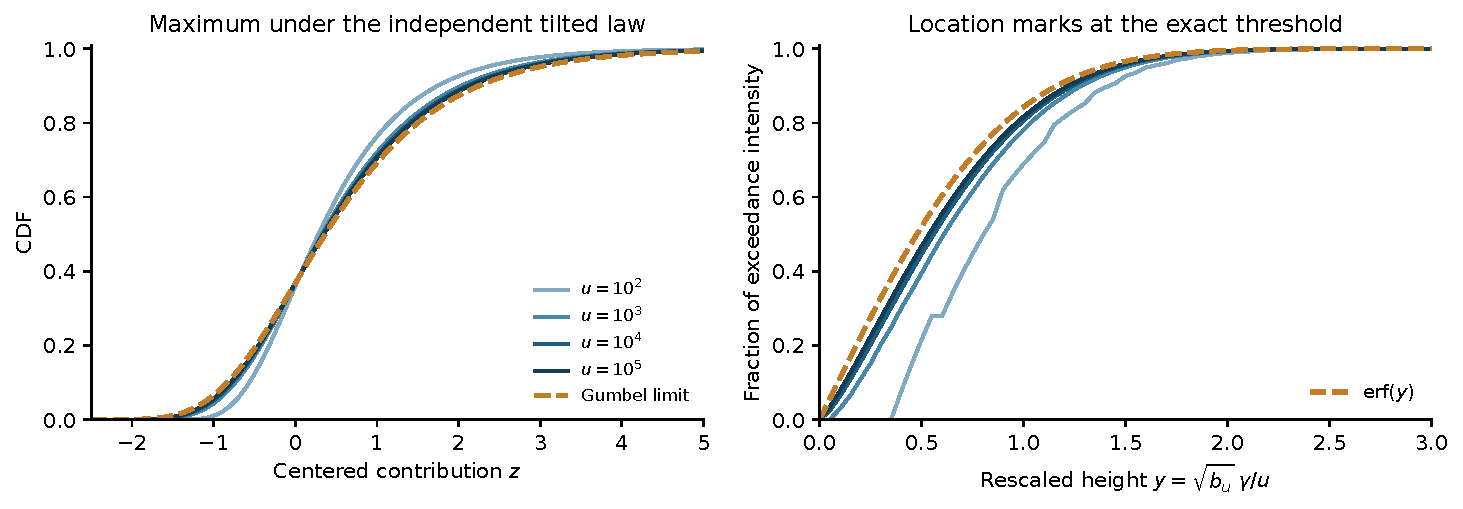
\includegraphics[width=\textwidth]{figures/tilted_extremes.pdf}
\caption{Deterministic diagnostics for the synthetic counting-law spectrum
with $\theta=1$. These panels use the independent tilted distribution,
which the proof transfers to the conditioned extreme process. The right
panel is the distribution of an exceedance's location mark at the exact
threshold, not a finite-sample winning-index distribution.}
\label{fig:diagnostics}
\end{figure}

For shape one, the numerical exact centers and their differences from
$b_0(u)=\log u+\tfrac12\log\log u-\log(4\sqrt\pi)$ are:
\begin{center}
\begin{tabular}{@{}rrrr@{}}
\toprule
$u$ & Exact center (numerical) & $b_u-b_0(u)$ & Maximum grid CDF error\\
\midrule
$10^2$ & $2.452817$ & $-0.957283$ & $0.074918$\\
$10^3$ & $5.293511$ & $-0.621907$ & $0.028470$\\
$10^4$ & $7.896763$ & $-0.465082$ & $0.018176$\\
$10^5$ & $10.401168$ & $-0.374833$ & $0.013517$\\
\bottomrule
\end{tabular}
\end{center}
The grid is $-2.5\le z\le5$ with spacing $0.1$. Slow convergence of the
explicit center is visible. The table is evidence for using the exact
normalization in finite computations; it is not an error bound for the
Dirichlet-zero application.

\subsection{Validation of the sharper centering formula}

For the same synthetic spectrum, the continuous counting approximation
\[
 N_0(T)=\frac{T}{2\pi}\left(\log\frac{T}{2\pi}-1\right)
\]
differs from the actual count by at most one, globally. Indeed, $N_0$
lies in $[-1,0]$ below $2\pi e$, and above this point the count is its
integer part. Proposition~\ref{ext:prop:refinedcenter} therefore gives
the analytic enclosure with $\varepsilon_u=e^{-B_u}$. The separate
script \texttt{code/refined\_center.py} computes $B_u$ and compares it
with the exact-center diagnostics already saved by the main experiment.
The root calculations use ordinary floating point; the theoretical
enclosure is proved analytically, while these numerical evaluations
are not interval arithmetic certificates.

\begin{table}[htbp]
\centering
\small
\begin{tabular}{rrrrr}
\hline
$u$ & Stored $b_{\rm num}$ & $|b_{\rm num}-b_{\rm elem}|$
    & $|b_{\rm num}-B|$ & $\varepsilon=e^{-B}$\\
\hline
$10^2$ & $2.4528173301$ & $9.5728\times10^{-1}$
       & $2.6162\times10^{-2}$ & $8.3829\times10^{-2}$\\
$10^3$ & $5.2935113136$ & $6.2191\times10^{-1}$
       & $2.2252\times10^{-3}$ & $5.0129\times10^{-3}$\\
$10^4$ & $7.8967627345$ & $4.6508\times10^{-1}$
       & $1.7295\times10^{-4}$ & $3.7188\times10^{-4}$\\
$10^5$ & $10.4011683936$ & $3.7483\times10^{-1}$
       & $1.4413\times10^{-5}$ & $3.0397\times10^{-5}$\\
\hline
\end{tabular}
\caption{Refined centering for $\theta=1$ on the synthetic inverse-count
spectrum $\gamma_j=2\pi j/W(j/e)$, reusing the stored numerical roots.
Here $b_{\rm elem}$ is the elementary logarithmic center and $B$ solves
\eqref{ext:eq:refinedroot}.  All four stored roots lie inside the
numerically evaluated enclosure
$[B+\log(1-\varepsilon),B+\log(1+\varepsilon)]$.
These are floating-point diagnostics, not interval-certified evaluations
or computations of actual zeta zeros.}
\label{ext:tab:refinedcenter}
\end{table}


\subsection{Exact conditional sampling for finite spectra}

The second experiment uses $\gamma_j=j$ for $1\le j\le n$, with
$(u,n)=(20,1000)$ and $(80,4000)$. This is a finite model. Set
$\mu=\sum_j[1+(j/u)^2]^{-1}$. Propose independent
$R_j\sim\mathrm{Exp}(1+(j/u)^2)$ and accept the vector with probability
\[
 e^{S-\mu}\mathbf1_{S\le\mu}.
\]
The change-of-measure identity proves that the accepted vector has
exactly the original finite exponential law conditioned on $S\le\mu$.
There is no Gaussian substitution for omitted coordinates. Each case has
6000 accepted vectors with fixed recorded seeds. Acceptance proportions
are approximately $0.1004$ and $0.0504$; the mean slacks are $0.9500$
and $0.9720$, approaching the unit-exponential mean. The finite sample
correlations need not vanish, and no finite-$u$ independence claim is made.

\begin{figure}[ht]
\centering
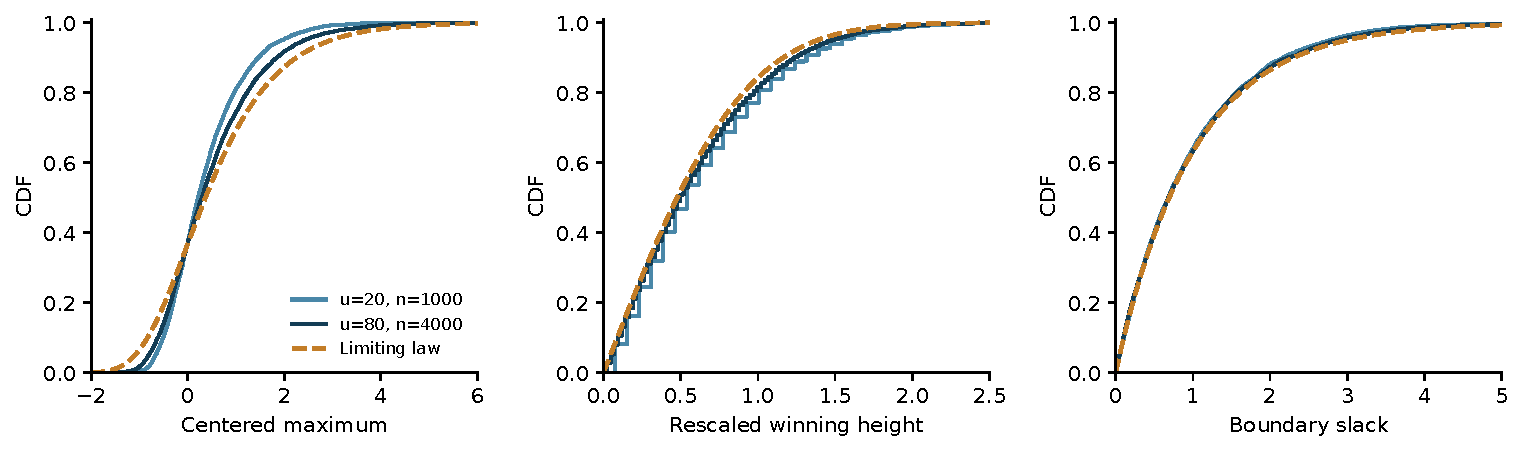
\includegraphics[width=\textwidth]{figures/conditional_experiment.pdf}
\caption{Empirical distribution functions from exact rejection sampling of
the stated finite conditional models, compared with their limiting shapes.
Finite truncation, finite saddle, and sampling error are all present. The
raw sampled observables and summary statistics are included in the archive.}
\end{figure}

\section{Formalization route and quantitative limits}

The archive contains a dependency plan rather than unverified Lean theorem
stubs. A formal development can first handle a general positive spectrum:
gamma product tilting; regular-variation summation; the uniform Fourier
local limit; the exact conditional density ratio; marked rare-event
convergence; and the functional bridge. Only the final identification of
the Laplace transform needs the completed Dirichlet product and the
upstream zero-location theorem. The cited source uses a separate Lean
toolchain from the main ProveIt article target; no connection between those
builds has been assumed for these new results.

Three limitations are mathematically substantive. First, arbitrary regular
variation gives no rate of convergence. The exact center is necessary
unless one controls the slowly varying factor on shrinking scales.
Second, the path uses its exact tilted mean; replacing that mean by its
leading asymptotic may introduce an error larger than the fluctuation
scale, as the source already demonstrates. Third, these results hold for
a fixed spectrum. Uniform conductor or degree bounds and effective
conditional convergence rates require further estimates. None is used
implicitly in the proof.

\begin{thebibliography}{99}
\small\raggedright

\bibitem{ProveIt2026}
V.~Reshetnikov, \emph{ProveIt: Generalized Riemann Hypothesis research
article and extensions}, snapshot
\texttt{00cadb961bbe77c74e5d082c4948f8884d58a970}, 27 November 2026.
Relevant source: \texttt{Article/sections/ana.tex}, especially
\texttt{ana:thm:condlaw}, \texttt{ana:thm:block},
\texttt{ana:thm:macro}, \texttt{ana:cor:fourfifths}, and
\texttt{ana:thm:medianheight}.
\url{https://github.com/VladimirReshetnikov/ProveIt/tree/00cadb961bbe77c74e5d082c4948f8884d58a970/Analysis/GeneralizedRiemannHypothesis}.

\bibitem{Sutherland2026}
A.~Sutherland, \emph{Verification files for the shorter Lean proof of RH
and of GRH for Dirichlet L-functions}, updated 27 November 2026;
upstream revision \texttt{72fead102f663d5c7a407964a13dc0cf9d977207}.
\url{https://math.mit.edu/~drew/shortgrh/}.

\bibitem{Bose2008}
A.~Bose, A.~Dasgupta, and K.~Maulik,
\emph{Maxima of Dirichlet and triangular arrays of gamma variables},
Statistics \& Probability Letters \textbf{78} (2008), 2811--2820.
\url{https://doi.org/10.1016/j.spl.2008.03.032};
\url{https://arxiv.org/abs/0803.3518}.

\bibitem{MayerWolf1993}
E.~Mayer-Wolf and O.~Zeitouni,
\emph{The probability of small Gaussian ellipsoids and associated
conditional moments}, Annals of Probability \textbf{21} (1993), 14--24.
\url{https://doi.org/10.1214/aop/1176989391}.

\bibitem{BGT1987}
N.~H.~Bingham, C.~M.~Goldie, and J.~L.~Teugels,
\emph{Regular Variation}, Encyclopedia of Mathematics and its
Applications, vol.~27, Cambridge University Press, 1987.
The uniform convergence theorem and standard regular-variation bounds
are used in the spectral summation arguments.

\bibitem{Whitt2007}
W.~Whitt, \emph{Proofs of the martingale FCLT},
Probability Surveys \textbf{4} (2007), 268--302.
\url{https://doi.org/10.1214/07-PS122};
\url{https://arxiv.org/abs/0712.1929}.

\bibitem{Bennett2021}
M.~A.~Bennett, G.~Martin, K.~O'Bryant, and A.~Rechnitzer,
\emph{Counting zeros of Dirichlet $L$-functions},
Mathematics of Computation \textbf{90} (2021), 1455--1482.
\url{https://doi.org/10.1090/mcom/3599};
\url{https://arxiv.org/abs/2005.02989}.

\bibitem{Gao2003}
F.~Gao, J.~Hannig, T.-Y.~Lee, and F.~Torcaso,
\emph{Laplace transforms via Hadamard factorization},
Electronic Journal of Probability \textbf{8} (2003), paper 13, 1--20.
\url{https://doi.org/10.1214/EJP.v8-151}.

\bibitem{Gyorgyi2003}
G.~Gy\"orgyi, P.~C.~W.~Holdsworth, B.~Portelli, and Z.~R\'acz,
\emph{Statistics of extremal intensities for Gaussian interfaces},
Physical Review E \textbf{68} (2003), 056116.
\url{https://doi.org/10.1103/PhysRevE.68.056116};
\url{https://arxiv.org/abs/cond-mat/0307645}.

\end{thebibliography}
\end{document}
